\subsection{UC10 - Rimozione della recensione rilasciata} \label{usecase:10}
\begin{figure}[H]
    \centering
    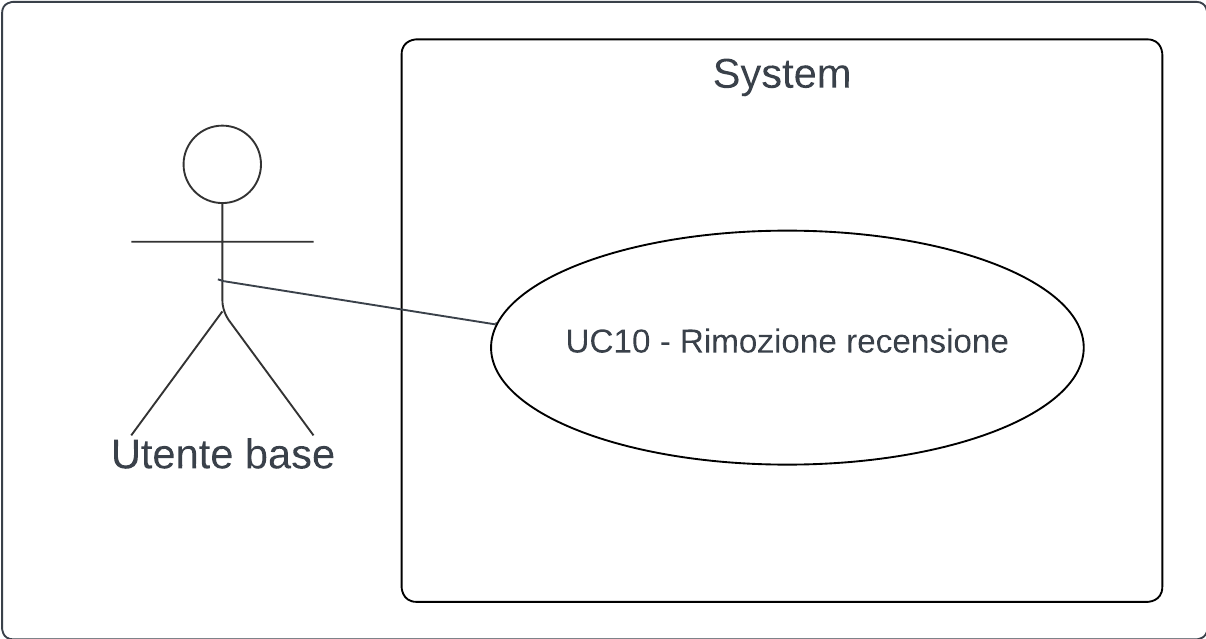
\includegraphics[width=0.75\linewidth]{ucd/UCD10.png}
\end{figure}
\textbf{Attori}:
\begin{itemize}
    \item Utente base
\end{itemize}
\textbf{Precondizioni}:
\begin{itemize}
    \item L'utente ha rilasciato in precedenza almeno una recensione (\nameref{usecase:7})
\end{itemize}
\textbf{Postcondizioni}:
\begin{itemize}
    \item L'utente ha rimosso la recensione desiderata
\end{itemize}
\textbf{\textit{Scenario}_G principale}:
\begin{enumerate}
    \item L'utente seleziona il ristorante che aveva recensito in precedenza
    \item L'utente seleziona la sua recensione pubblicata in precedenza
    \item L'utente rimuove la recensione selezionata
\end{enumerate}
\newpage